\documentclass[14pt]{beamer}
\usepackage{fontspec}
\usepackage{color}
\usepackage{minted}

%% These fonts are non-free.
%% Comment out the lines if you don't have them.
\setmainfont{Equity Text A}
\setsansfont{Concourse T3}
\setmonofont{Triplicate T4}

\definecolor{bgcolor}{RGB}{20,25,28}
\setbeamercolor{background canvas}{bg=bgcolor}
\setbeamercolor{normal text}{fg=white}
\setbeamercolor{itemize item}{fg=white}
\setbeamertemplate{itemize items}[circle]
\usemintedstyle{monokai}

\renewcommand{\theFancyVerbLine}{\color{darkgray}\large \oldstylenums{\arabic{FancyVerbLine}}}
\newcommand{\toptitle}[1]{
  {\huge #1} \\
  \vspace{0.2cm}
}
\renewcommand{\subtitle}[1]{
  {\large #1} \\
  \vspace{0.2cm}
}

\begin{document}
\begin{frame}
  \begin{center}
    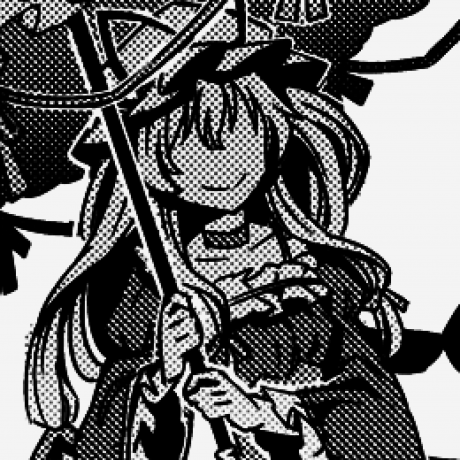
\includegraphics[height=4cm]{avatar.png}\\
    \vspace{0.2cm}
    {\Large Nicolas Hafner} \\
    \vspace{0.2cm}
    {\Huge @Shinmera} \\
    \vspace{0.2cm}
    \url{https://everything.shinmera.com}
  \end{center}
\end{frame}

\begin{frame}
  \toptitle{Last Year...}
  \begin{itemize}
  \item Qtools makes using Qt from CL neat
    \pause
  \item But Qt itself is awkward sometimes:
  \item Layouts are lacklustre
  \item Some features can't be changed
  \item Widgets are not extensible enough
  \end{itemize}
\end{frame}

\begin{frame}
  \toptitle{What to Do?}
  \begin{itemize}
  \item Qt sources can't feasibly be changed
  \item There's no way to hack fixes in otherwise
    \pause
  \item So we need to rewrite it all
  \item but this time in Lisp! \pause \quad\textbackslash o/
  \end{itemize}
\end{frame}

\begin{frame}
  \toptitle{Enter Qtools-UI}
  \begin{itemize}
  \item Offers a new, dynamic layouting protocol
  \item Implements a few standard layouts and widgets
  \item Includes useful base-classes to work with
  \item And completely pre-made components
  \end{itemize}
\end{frame}

\begin{frame}
  \toptitle{Things Like...}
  \begin{center}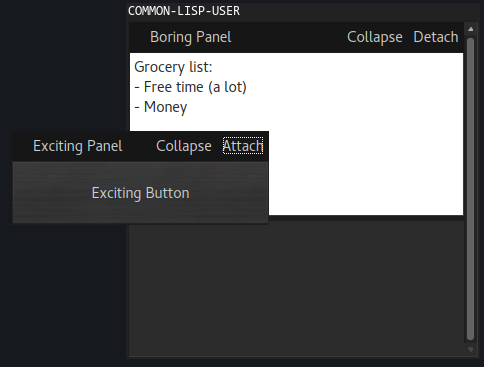
\includegraphics[height=6cm]{panels.png}\end{center}
\end{frame}

\begin{frame}
  \begin{center}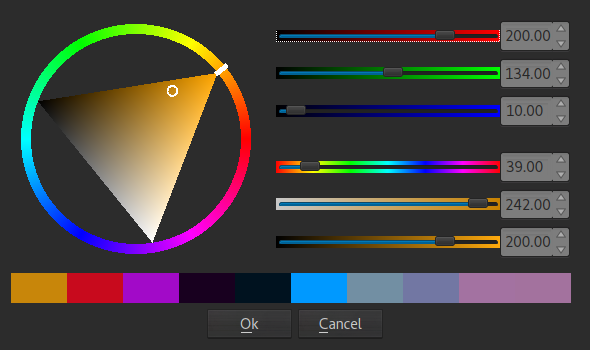
\includegraphics[height=5cm]{colors.png}\end{center}
\end{frame}

\begin{frame}
  \begin{center}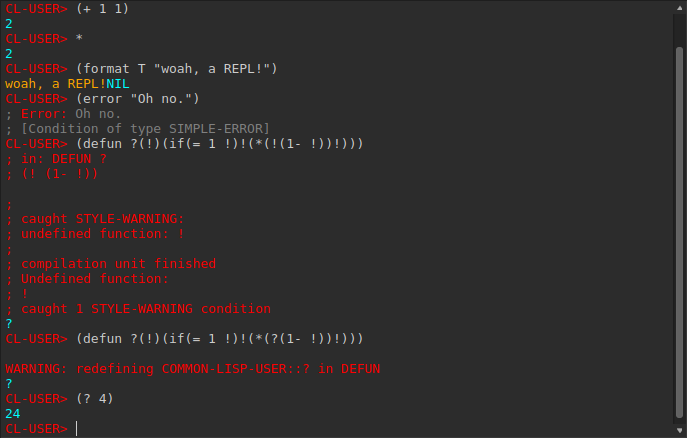
\includegraphics[height=7cm]{repl.png}\end{center}
\end{frame}

\begin{frame}
  \begin{center}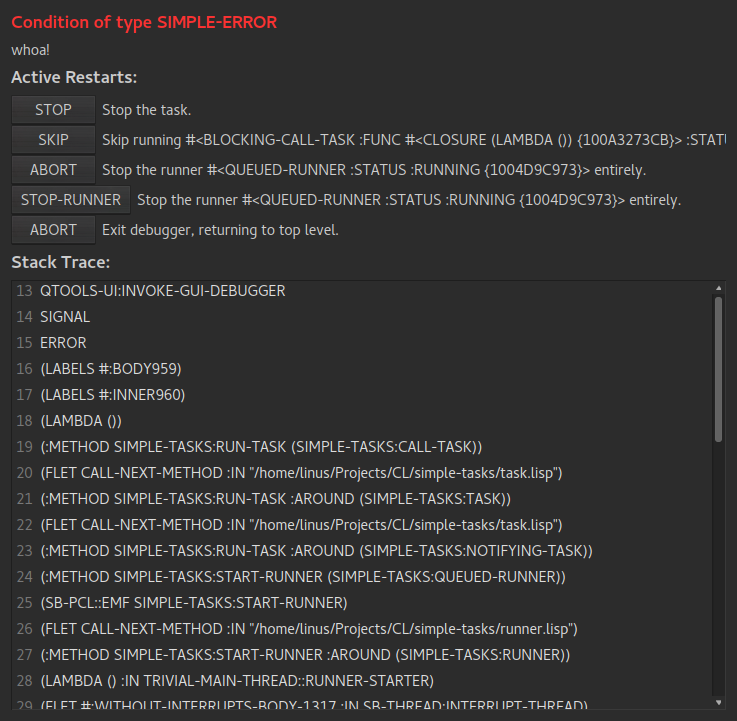
\includegraphics[height=8cm]{debugger.png}\end{center}
\end{frame}

\begin{frame}
  \toptitle{What's Next?}
  \begin{itemize}
  \item More layouts
  \item More components
    \pause
  \item More everything!
    \pause
  \item More extensive testing needed
  \item Contributors are more than welcome
  \end{itemize}
\end{frame}

\begin{frame}
  \begin{center}
    \colorbox{white}{
\includegraphics[height=3cm]{qtools-ui-logo.png}} \\
    {\small\bfseries \url{https://shinmera.github.io/qtools-ui}} \\
    \vspace{0.3cm}
    {\Large Available on Quicklisp}
  \end{center}
\end{frame}
\end{document}

%%% Local Variables:
%%% mode: latex
%%% TeX-command-extra-options: "-shell-escape"
%%% TeX-master: t
%%% TeX-engine: luatex
%%% End:
